\documentclass[a4paper, UTF8]{ctexrep}
\usepackage{ctex}
\usepackage{amsmath}
\usepackage{multirow}
\usepackage{amssymb}
\usepackage{graphicx}
\usepackage{geometry}
\usepackage{bm}
\usepackage{subfigure}
\usepackage{float}

\renewcommand\thesection{\arabic{section}}

\begin{document}
	\begin{titlepage}
		\centering
		\vspace{6cm}
		\LARGE{图像处理中的数学方法第一次作业报告}\\
		\vspace{3cm}
		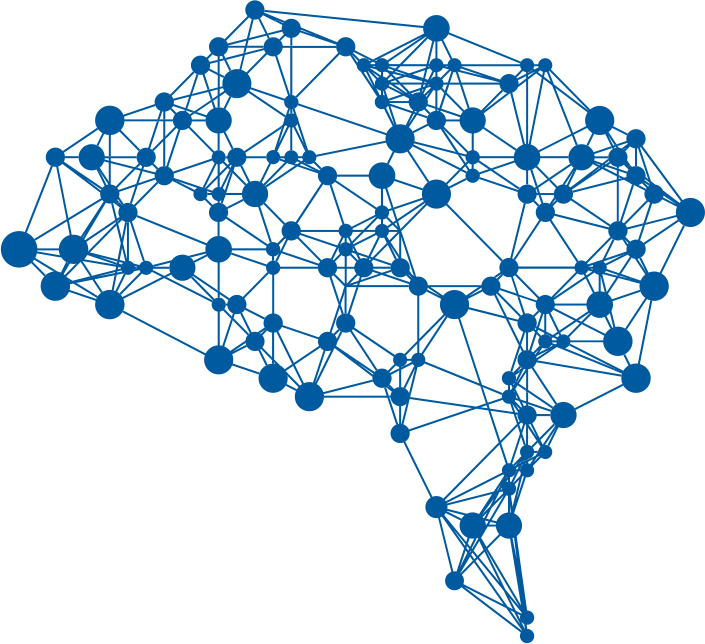
\includegraphics[width=0.8\textwidth]{deepLearning.png}\\
		\vspace{4cm}
		\normalsize{安捷 1601210097}\\
		\normalsize{\today}
	\end{titlepage}
	为了实现本次作业的需求,我基于MATLAB,实现了ADMM算法,利用迭代方法实现了去模糊+去噪的图像重建任务。下面从算法简述,参数设置,数值实验结果,结论四个方面总结本次作业。
	\section{算法简述}
		\begin{figure}
			\centering
			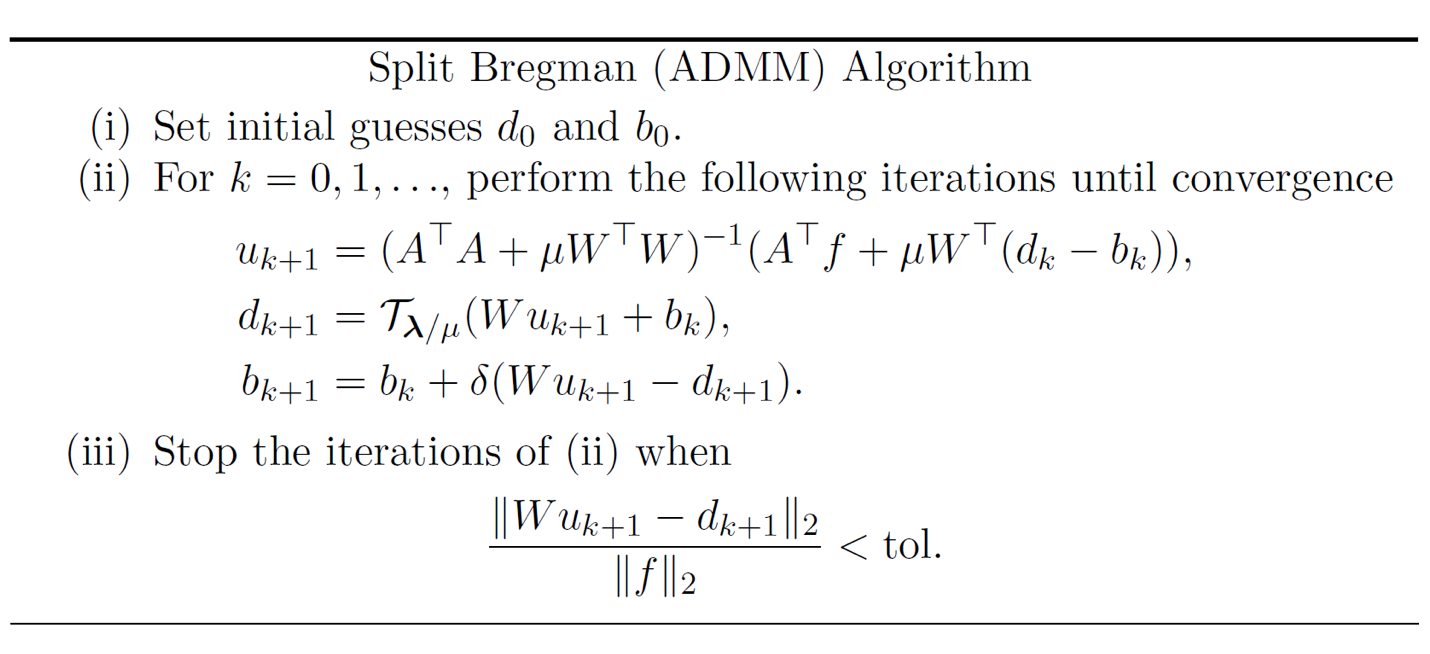
\includegraphics[width=0.8\textwidth]{fig1.png}
			\caption{算法流程}
		\end{figure}
		其中,主要问题在于第一步,在这次作业的开始,我尝试使用线性化的思路来实现本次作业,即,将 $A$算子与 $W$算子实现的操作转化为一个矩阵,经过线性化之后,上述流程中的操作全部转化为矩阵与向量的操作,这一操作可行,但是存在很严重的两个问题:
		\begin{enumerate}
			\item 存储困难,线性化的操作使得矩阵 $A$ 与$W$ 的维数是原图像的平方,即128*128的图像需要的双精度存储量为约1200MB,512*512的图像需要的双精度存储量为约80GB,如果不采取稀疏矩阵存储方式,几乎不可存储;
			\item 计算耗时长,在我使用的基于NVIDIA CUDA的GPU加速技术之后,依然速度很慢,主要原因在于矩阵求逆操作到目前为止没有效率很高的快速计算方法,即使采用GPU加速技术;
		\end{enumerate}
		基于以上两点原因,我放弃了这一方法,转为采用老师上课提到的利用Fourier Transform求解Possion方程的算法来求解ADMM算法的第一步。下面将算法简述如下:
		首先,原问题可以表述为:
		\begin{equation}
			\left( A^T A - \mu W^T W \right) u = M
		\end{equation}
		即有:
		\begin{equation}
			A * A * u - \mu L * u = M
		\end{equation}
		其中,L是拉普拉斯卷积核,上式经过FFT之后,有:
		\begin{equation}
			\hat A .* \hat A .* \hat u - \mu \hat L .* \hat u = \hat M
		\end{equation}
		即有:
		\begin{equation}
			\hat u = \frac{\hat M}{\hat A .* \hat A - \mu \hat L}
		\end{equation}
		\begin{equation}
			u = \mathrm{ifft2} \left( \frac{\mathrm{fft2} \left( M \right)}{\hat A .* \hat A - \mu \hat L} \right)
		\end{equation}
		上式即我在程序中实际应用的ADMM第一步求解方法。
		\section{参数设置}
			\begin{table}[htbp!]
				\centering
				\begin{tabular}{cc}
				\hline
				参数名称 & 参数值 \\
				\hline
				KERNEL\_SIZE & 15 \\
				SHIFT\_LEN & (KERNEL\_SIZE - 1) / 2 \\
				SIGMA & 1.5/2 \\
				SCALE & 100/200 \\
				MU & 0.3 \\
				LAMBDA & 0.06 \\
				TAU & LAMBDA / MU \\
				TOL & 1e-3 \\
				DELTA & 0.12 \\
				MAX\_ITERATION & 300 \\
				\hline
				\end{tabular}
				\caption{参数设置}
			\end{table}
			\section{数值实验结果}
				针对 $SIGMA = 1.5/2.0$ 及 $SCALE = 100/200$ 两组参数共四种情况,我分别进行了数值实验,其余参数均按照上一节的参数表设置,选取512*512 lena图进行数值实验,结果图示如下,其中original image为原始未经任何处理的图像,filtered image为按照作业要求,进行高斯平滑处理,并添加正太随机噪声的图像,reconstruction image为经过ADMM算法恢复之后的图像,error为按照作业要求进行误差度量得到的每次迭代误差分布:
				\begin{figure}[htbp!]
					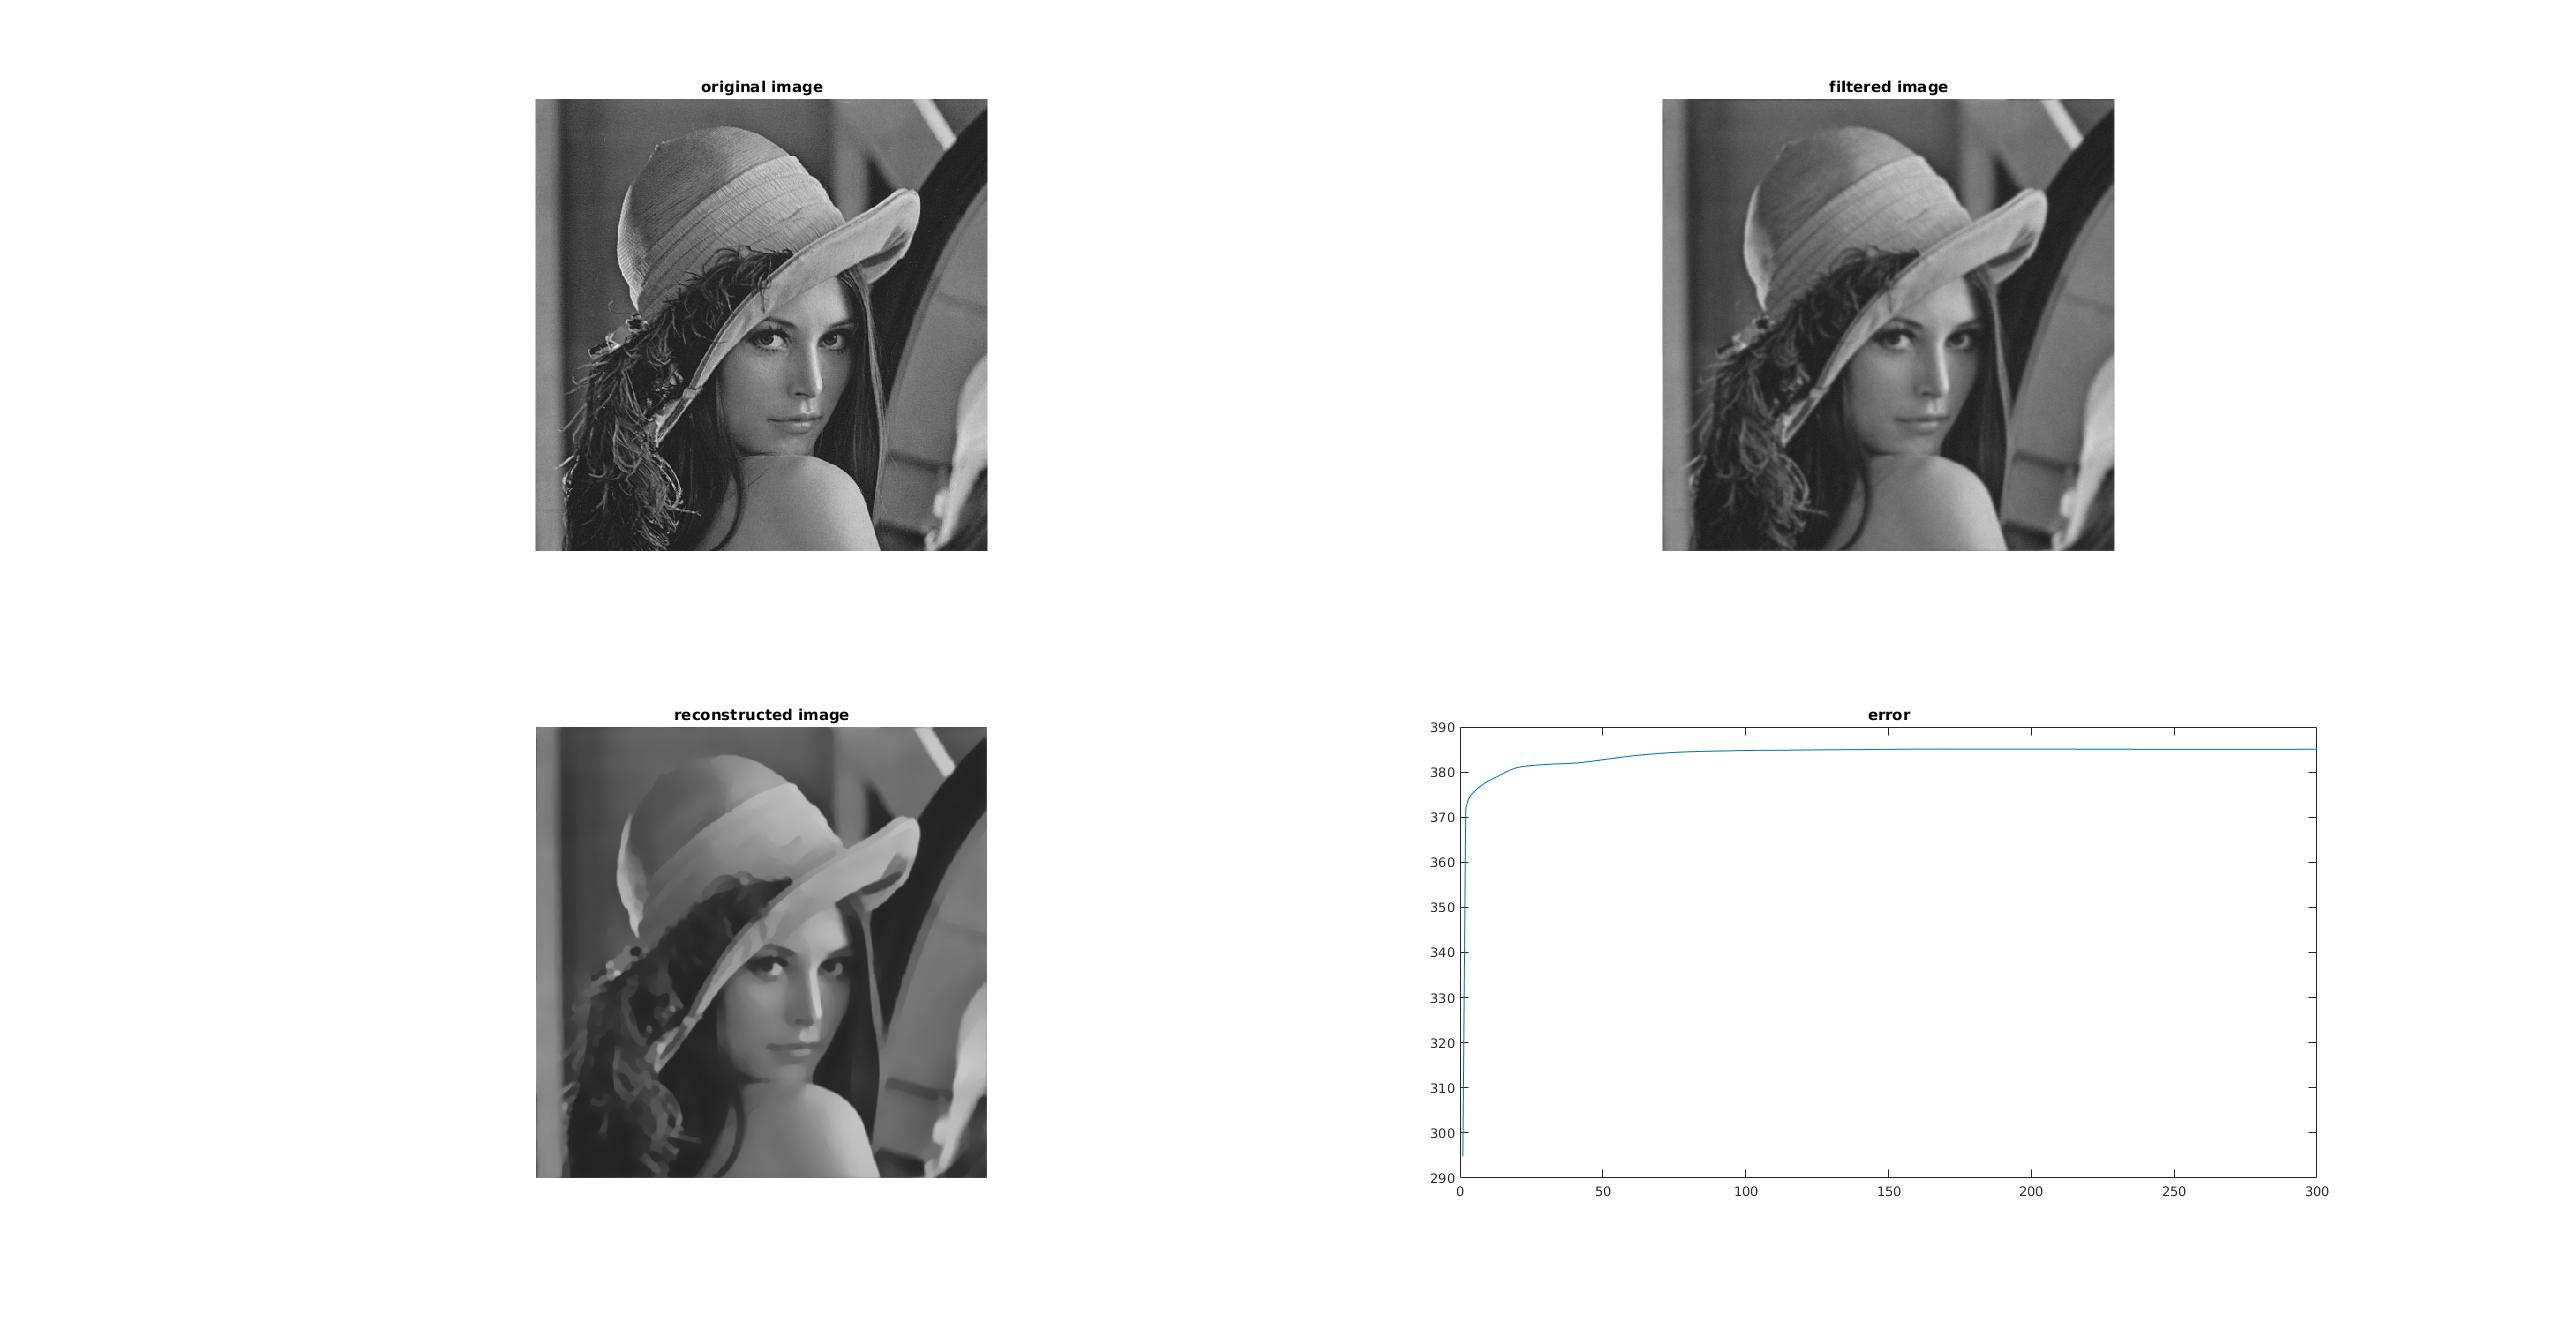
\includegraphics[width = 1 \textwidth]{fig2.jpg}
					\caption{SIGMA=1.5,SCALE=100 数值实验结果}
				\end{figure}
				\begin{figure}[htbp!]
					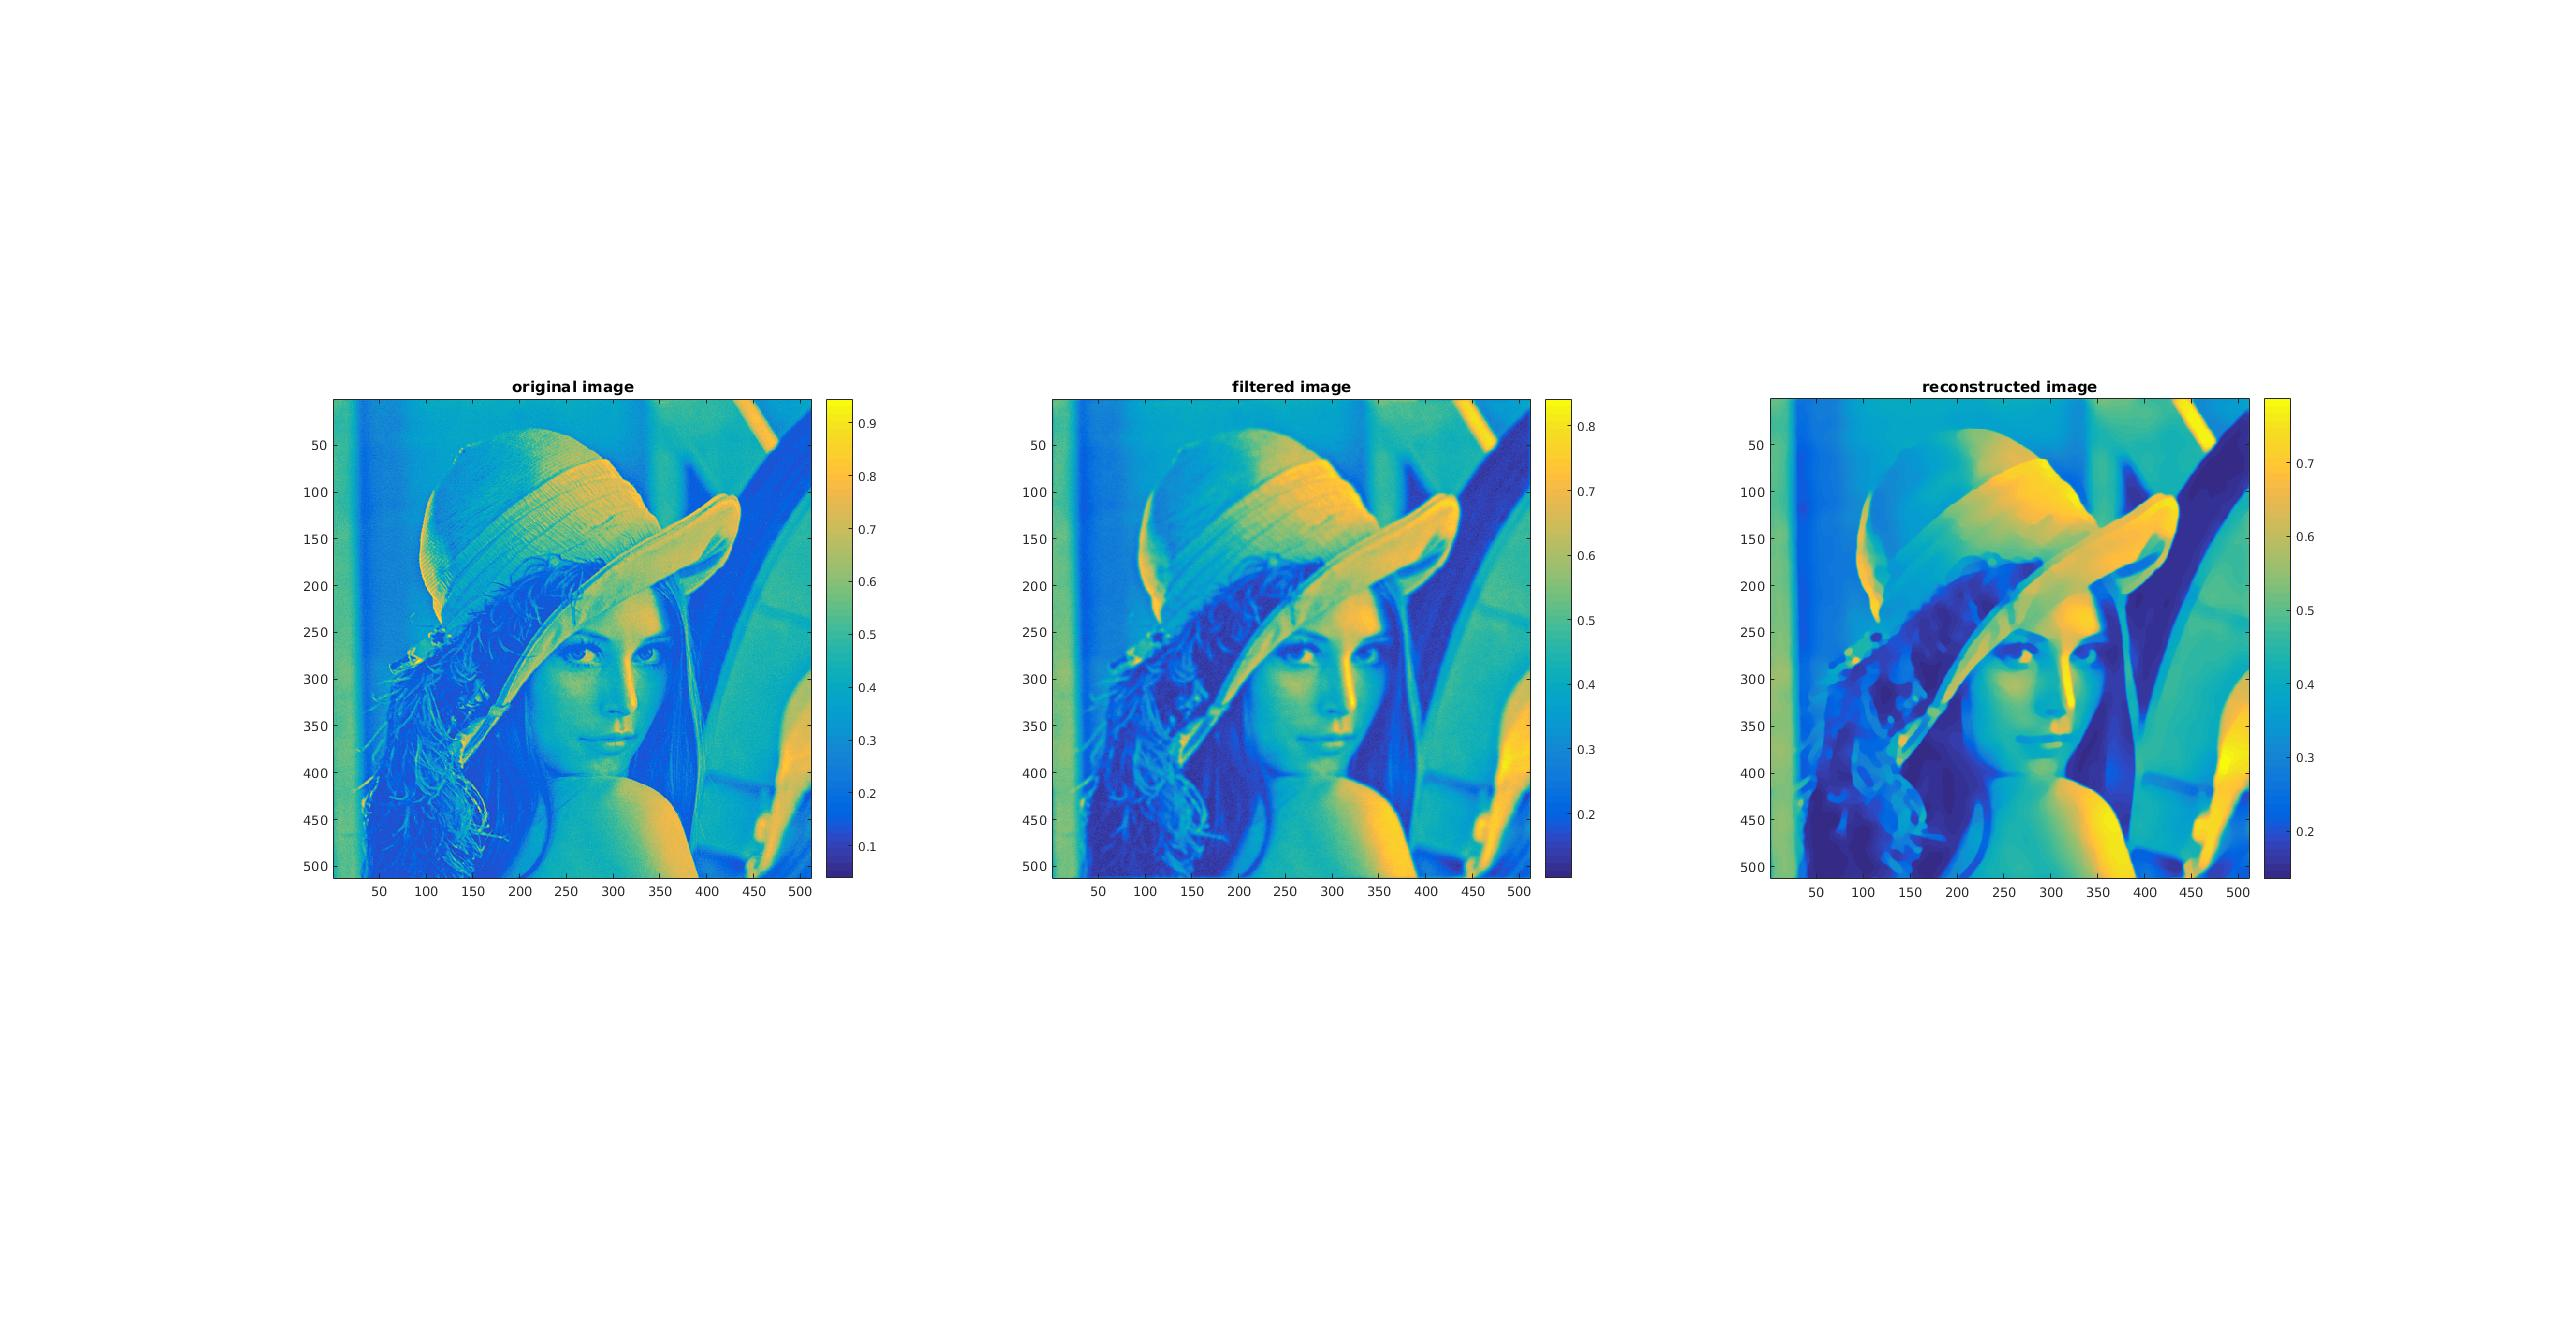
\includegraphics[width = 1 \textwidth]{fig3.jpg}
					\caption{SIGMA=1.5,SCALE=100 数值实验结果}
				\end{figure}
				\begin{figure}[htbp!]
					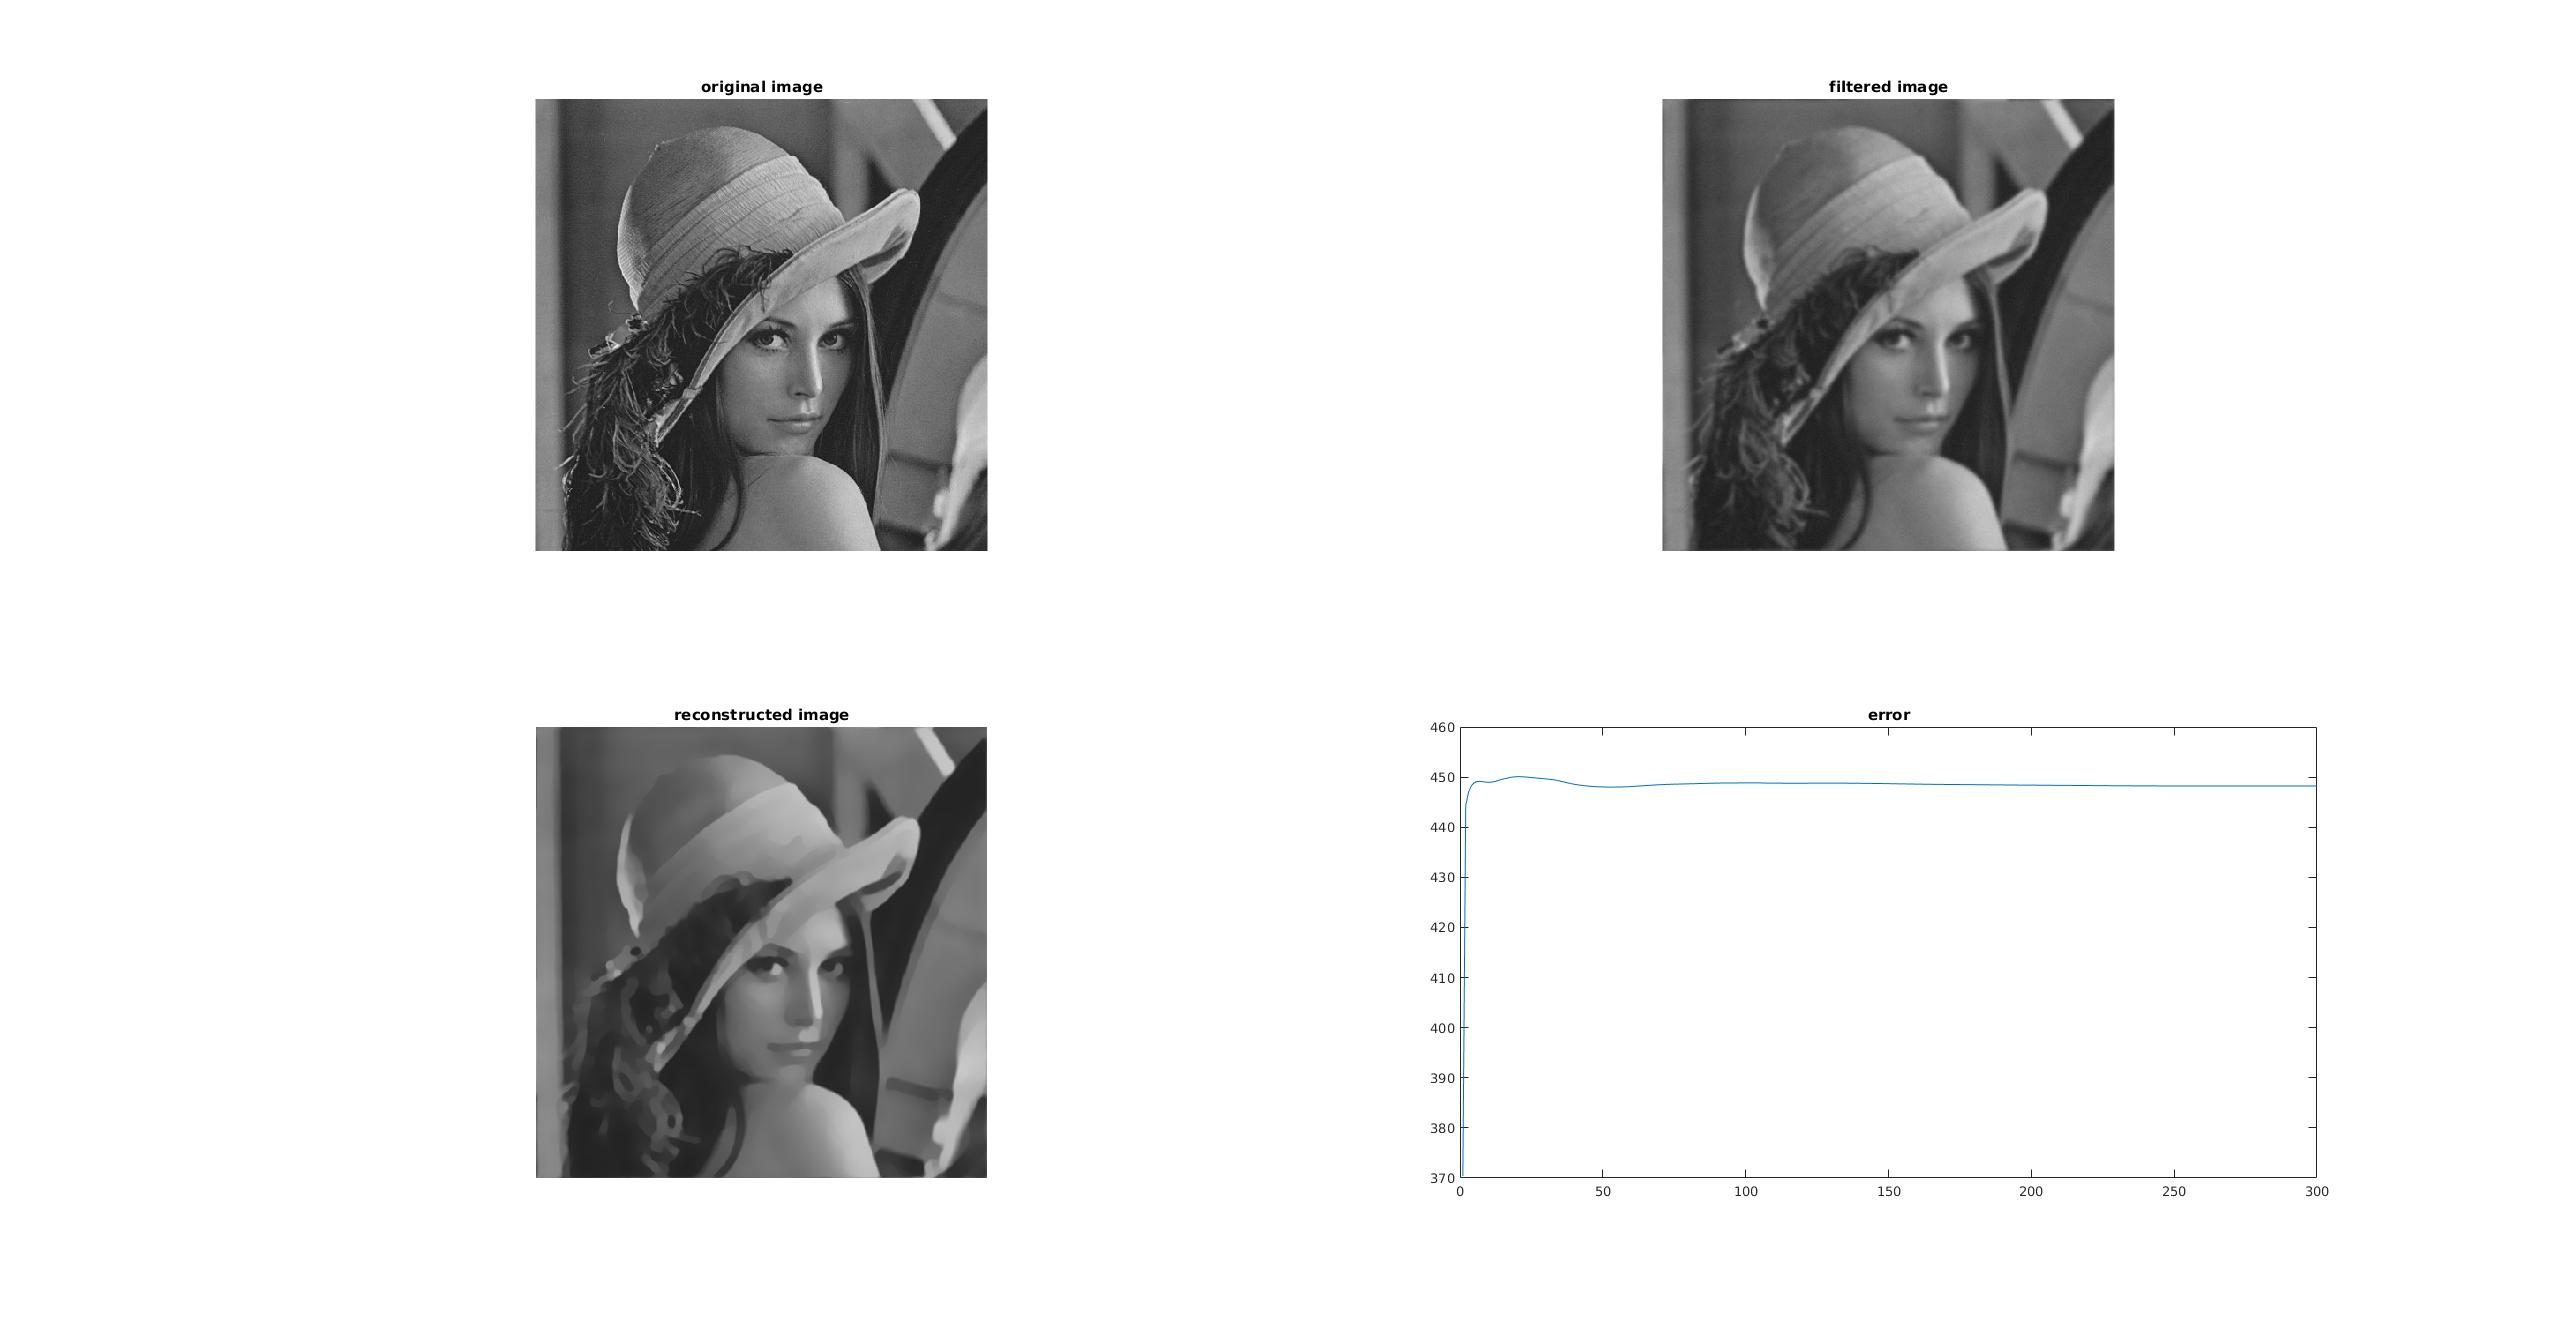
\includegraphics[width = 1 \textwidth]{fig4.jpg}
					\caption{SIGMA=2.0,SCALE=100 数值实验结果}
				\end{figure}
				\begin{figure}[htbp!]
					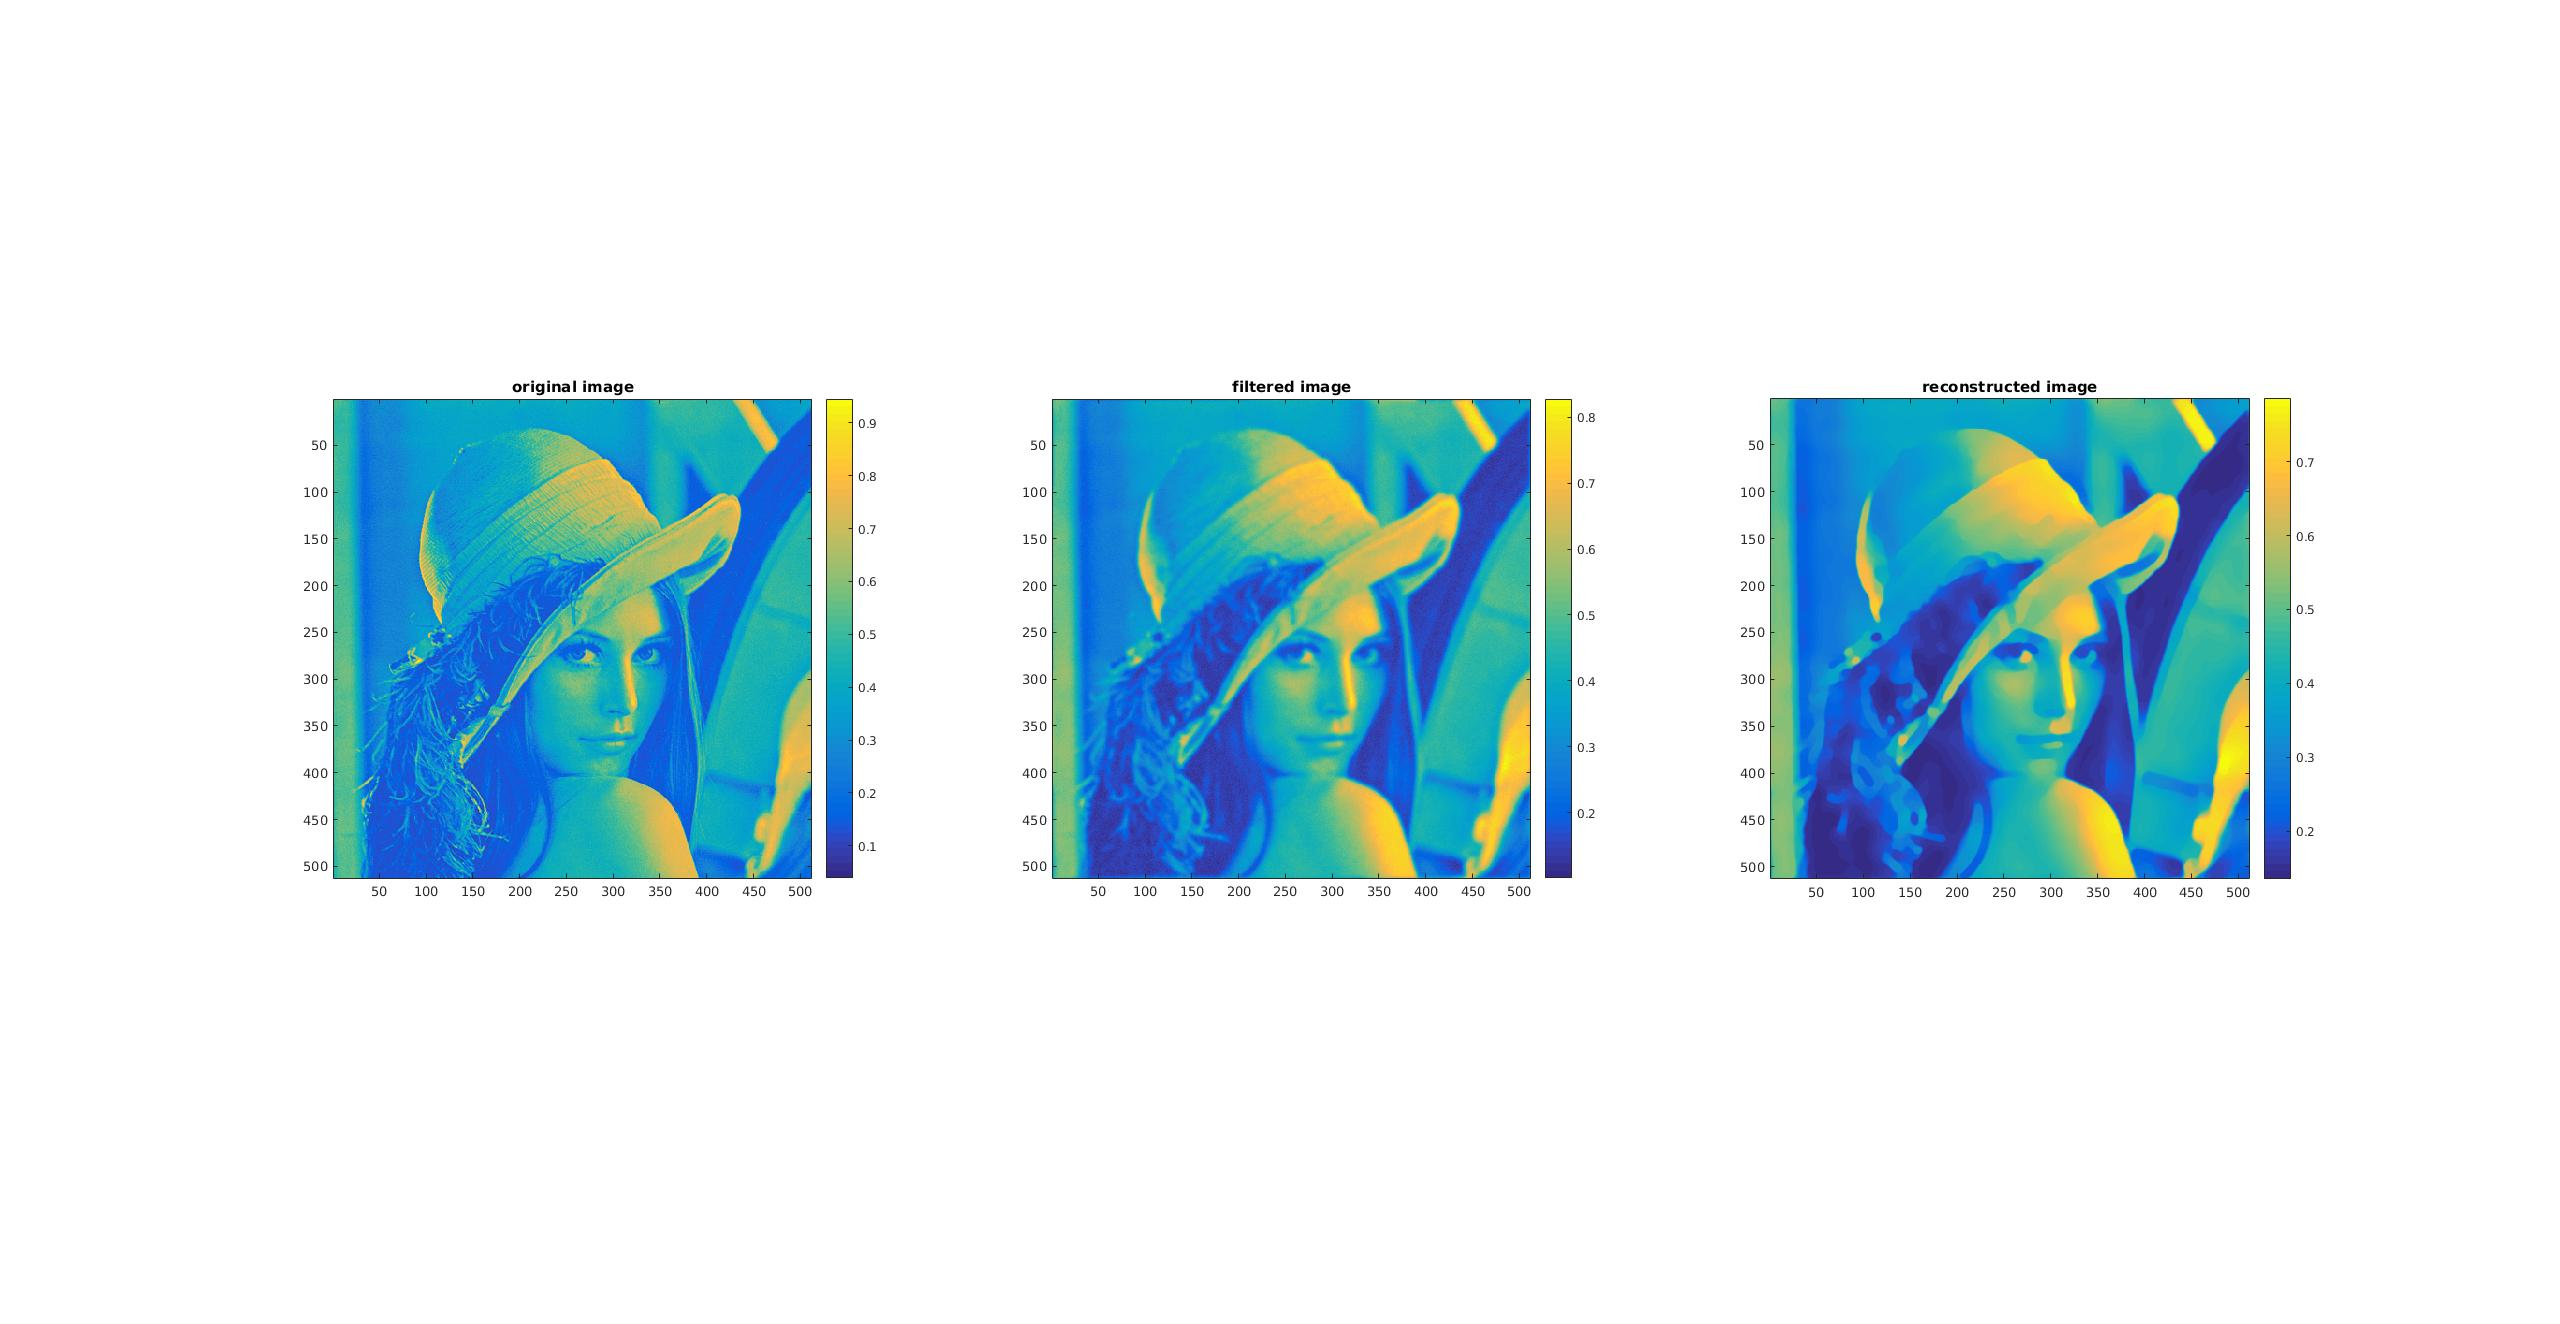
\includegraphics[width = 1 \textwidth]{fig5.jpg}
					\caption{SIGMA=2.0,SCALE=100 数值实验结果}
				\end{figure}
				\begin{figure}[htbp!]
					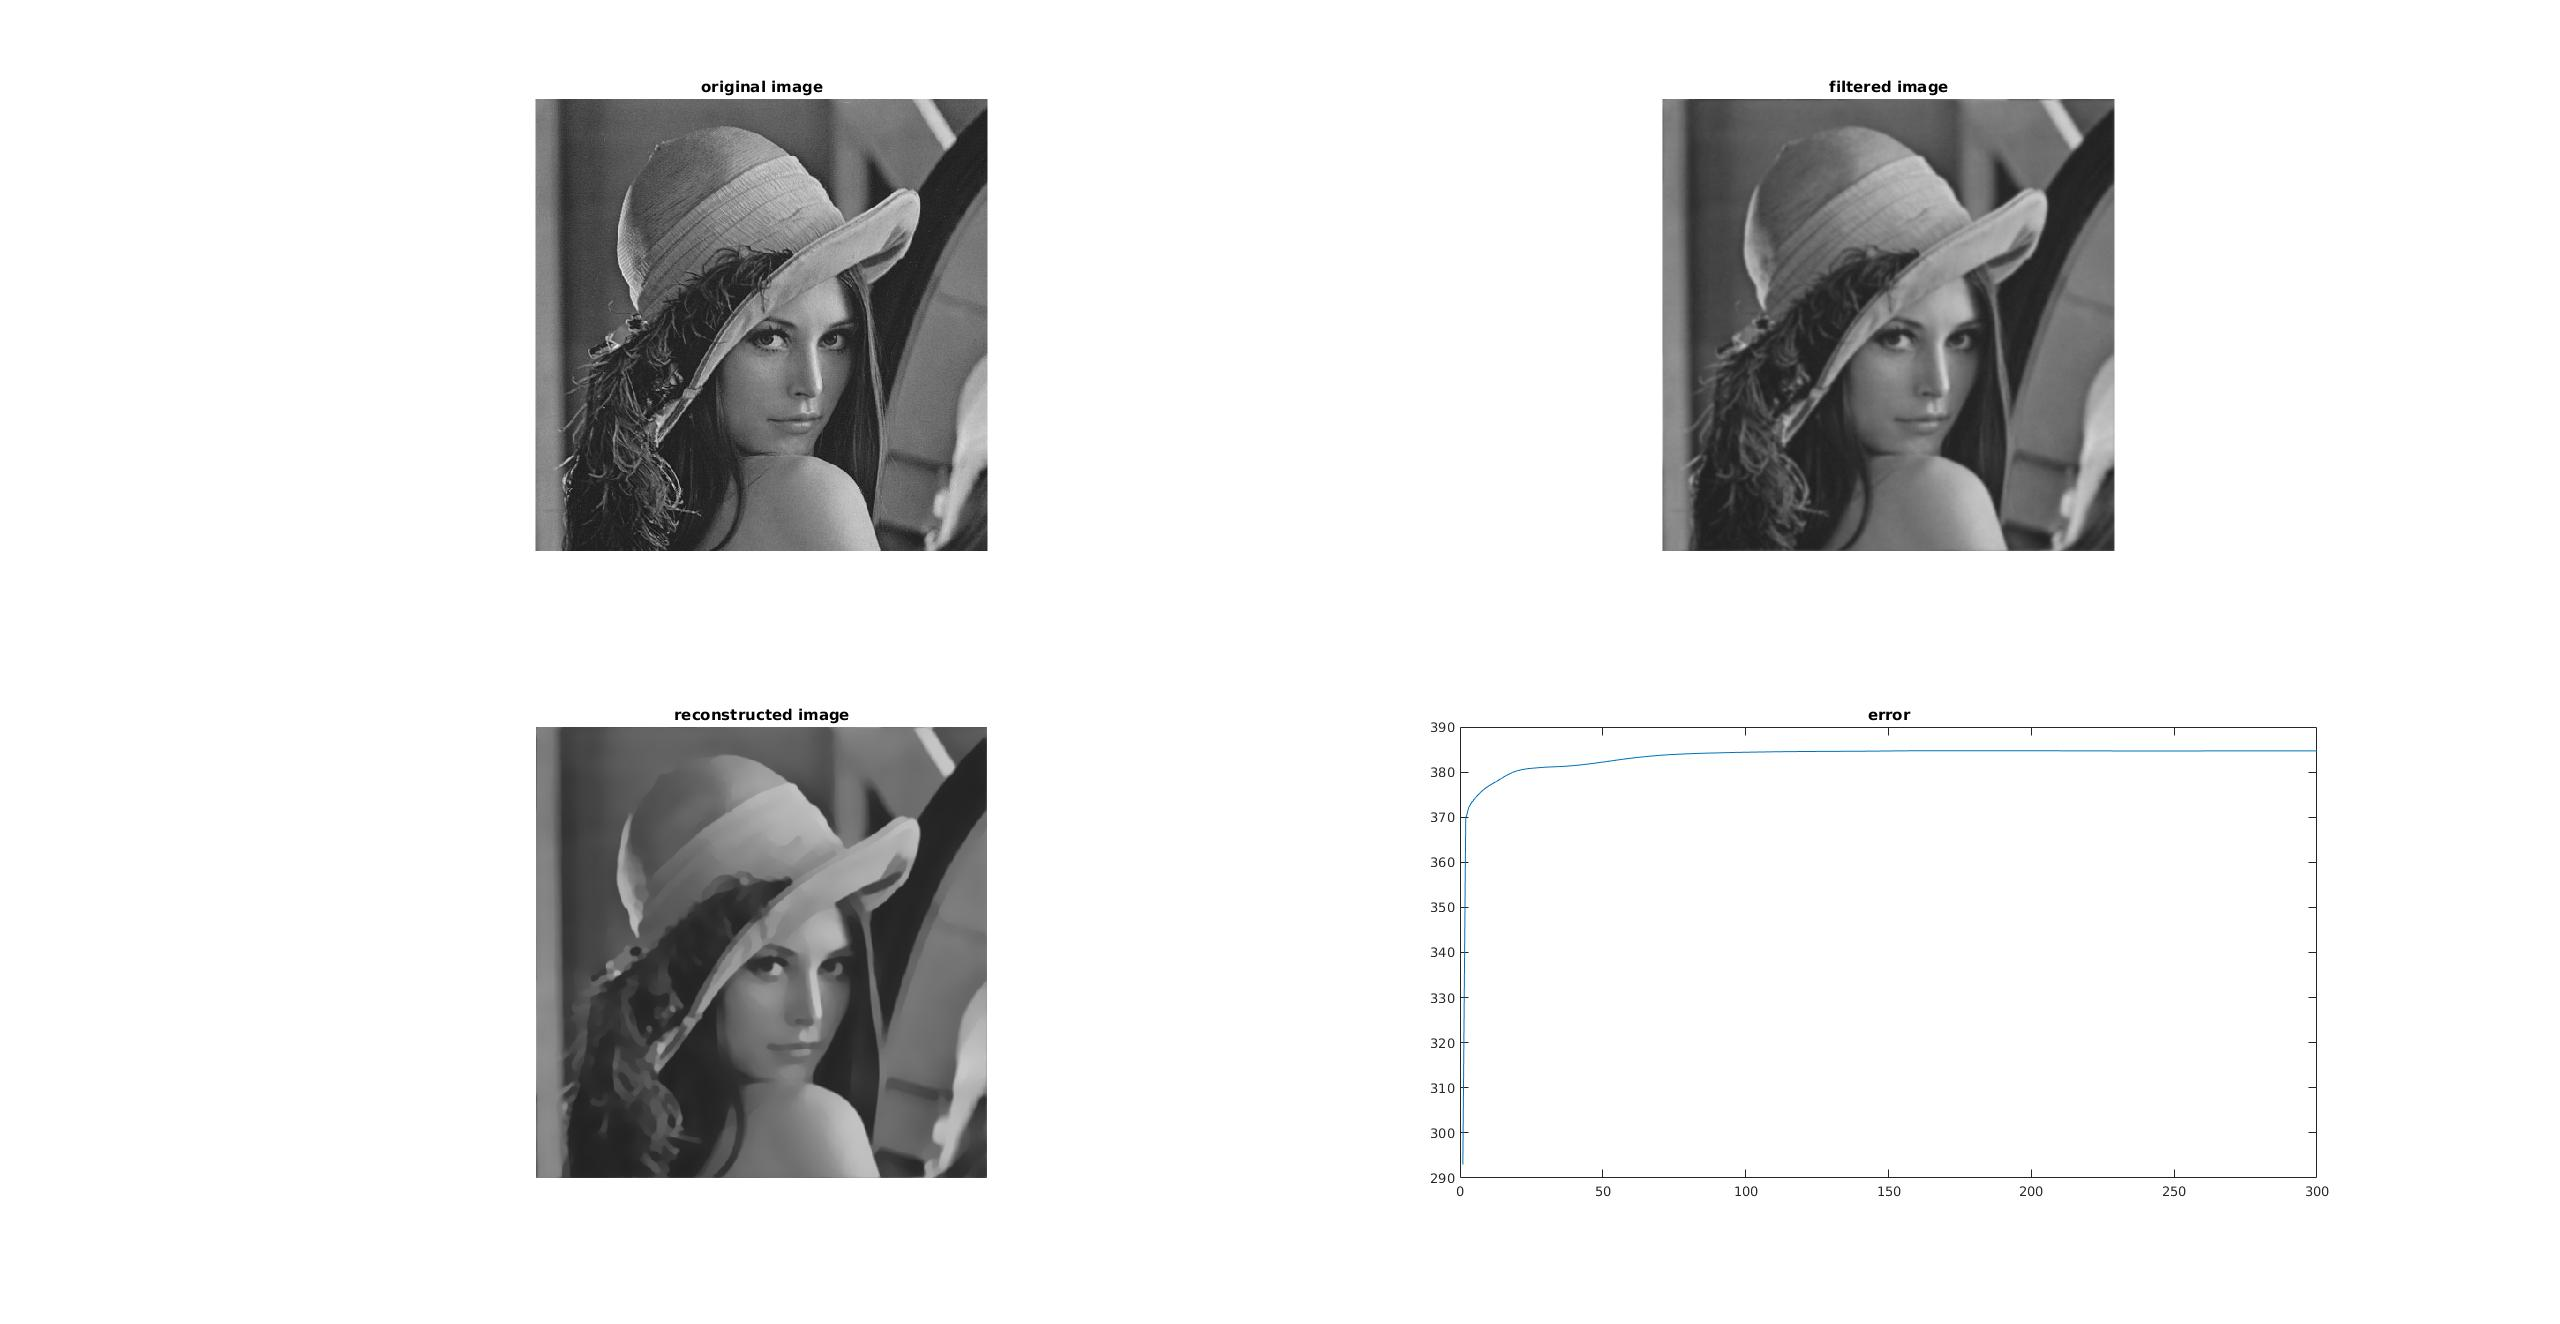
\includegraphics[width = 1 \textwidth]{fig6.jpg}
					\caption{SIGMA=1.5,SCALE=200 数值实验结果}
				\end{figure}
				\begin{figure}[htbp!]
					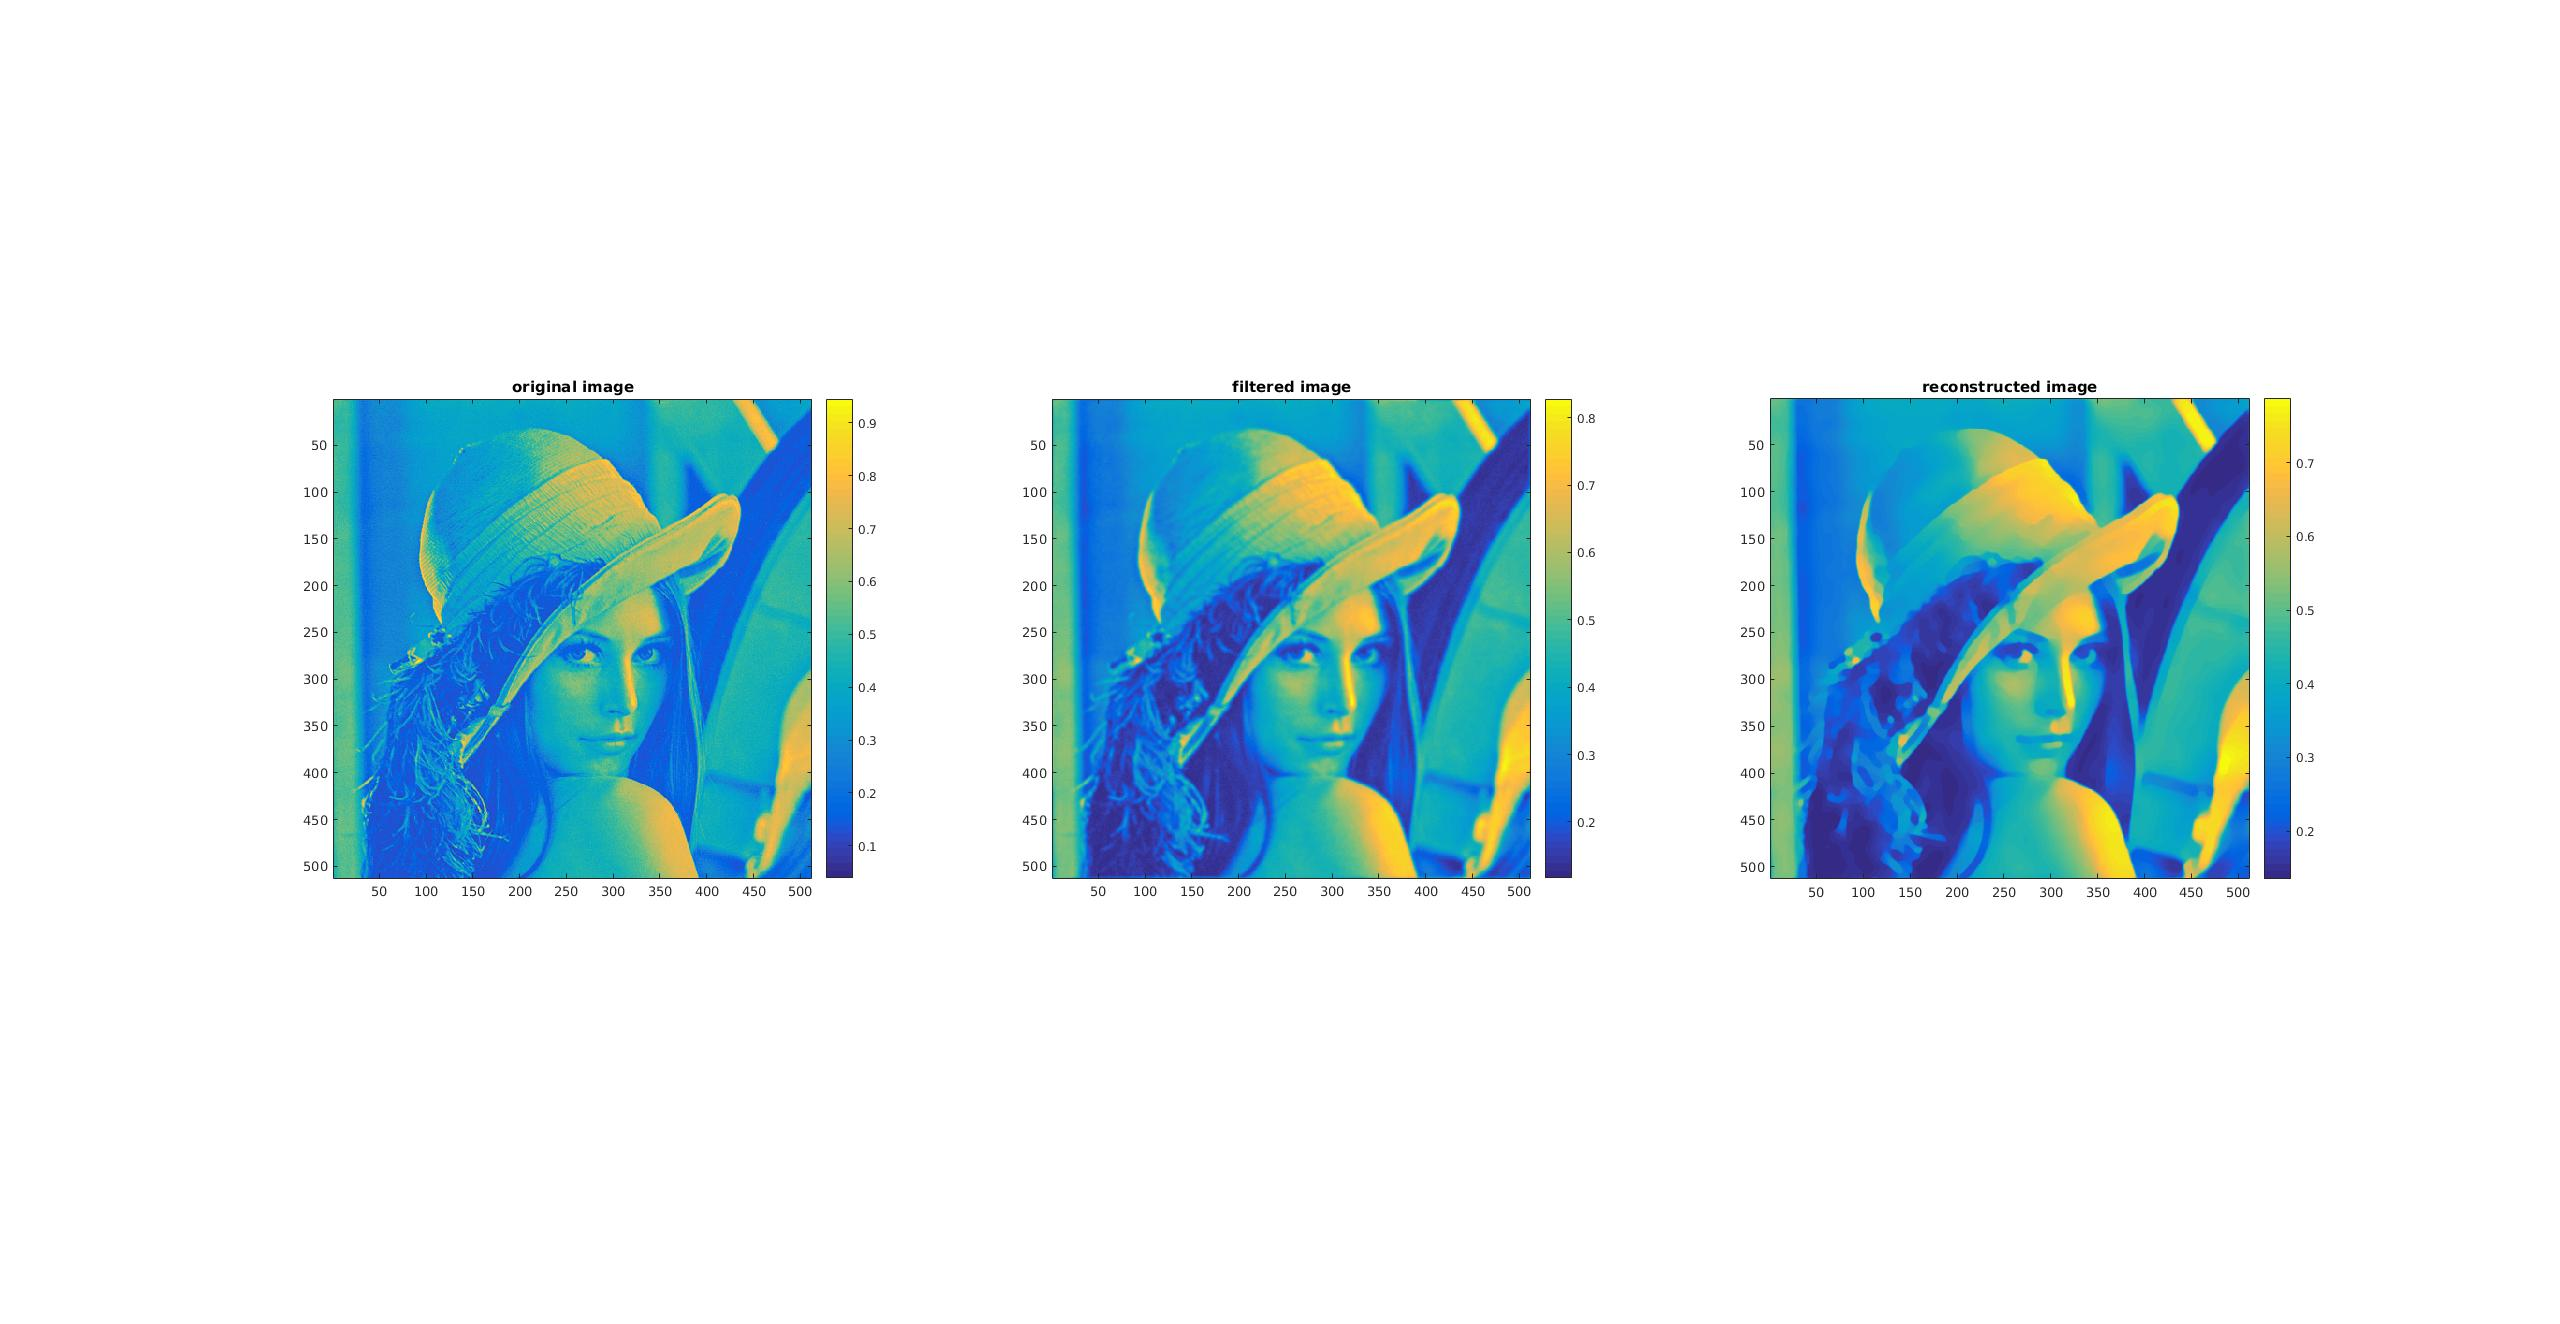
\includegraphics[width = 1 \textwidth]{fig7.jpg}
					\caption{SIGMA=1.5,SCALE=200 数值实验结果}
				\end{figure}
				\begin{figure}[htbp!]
					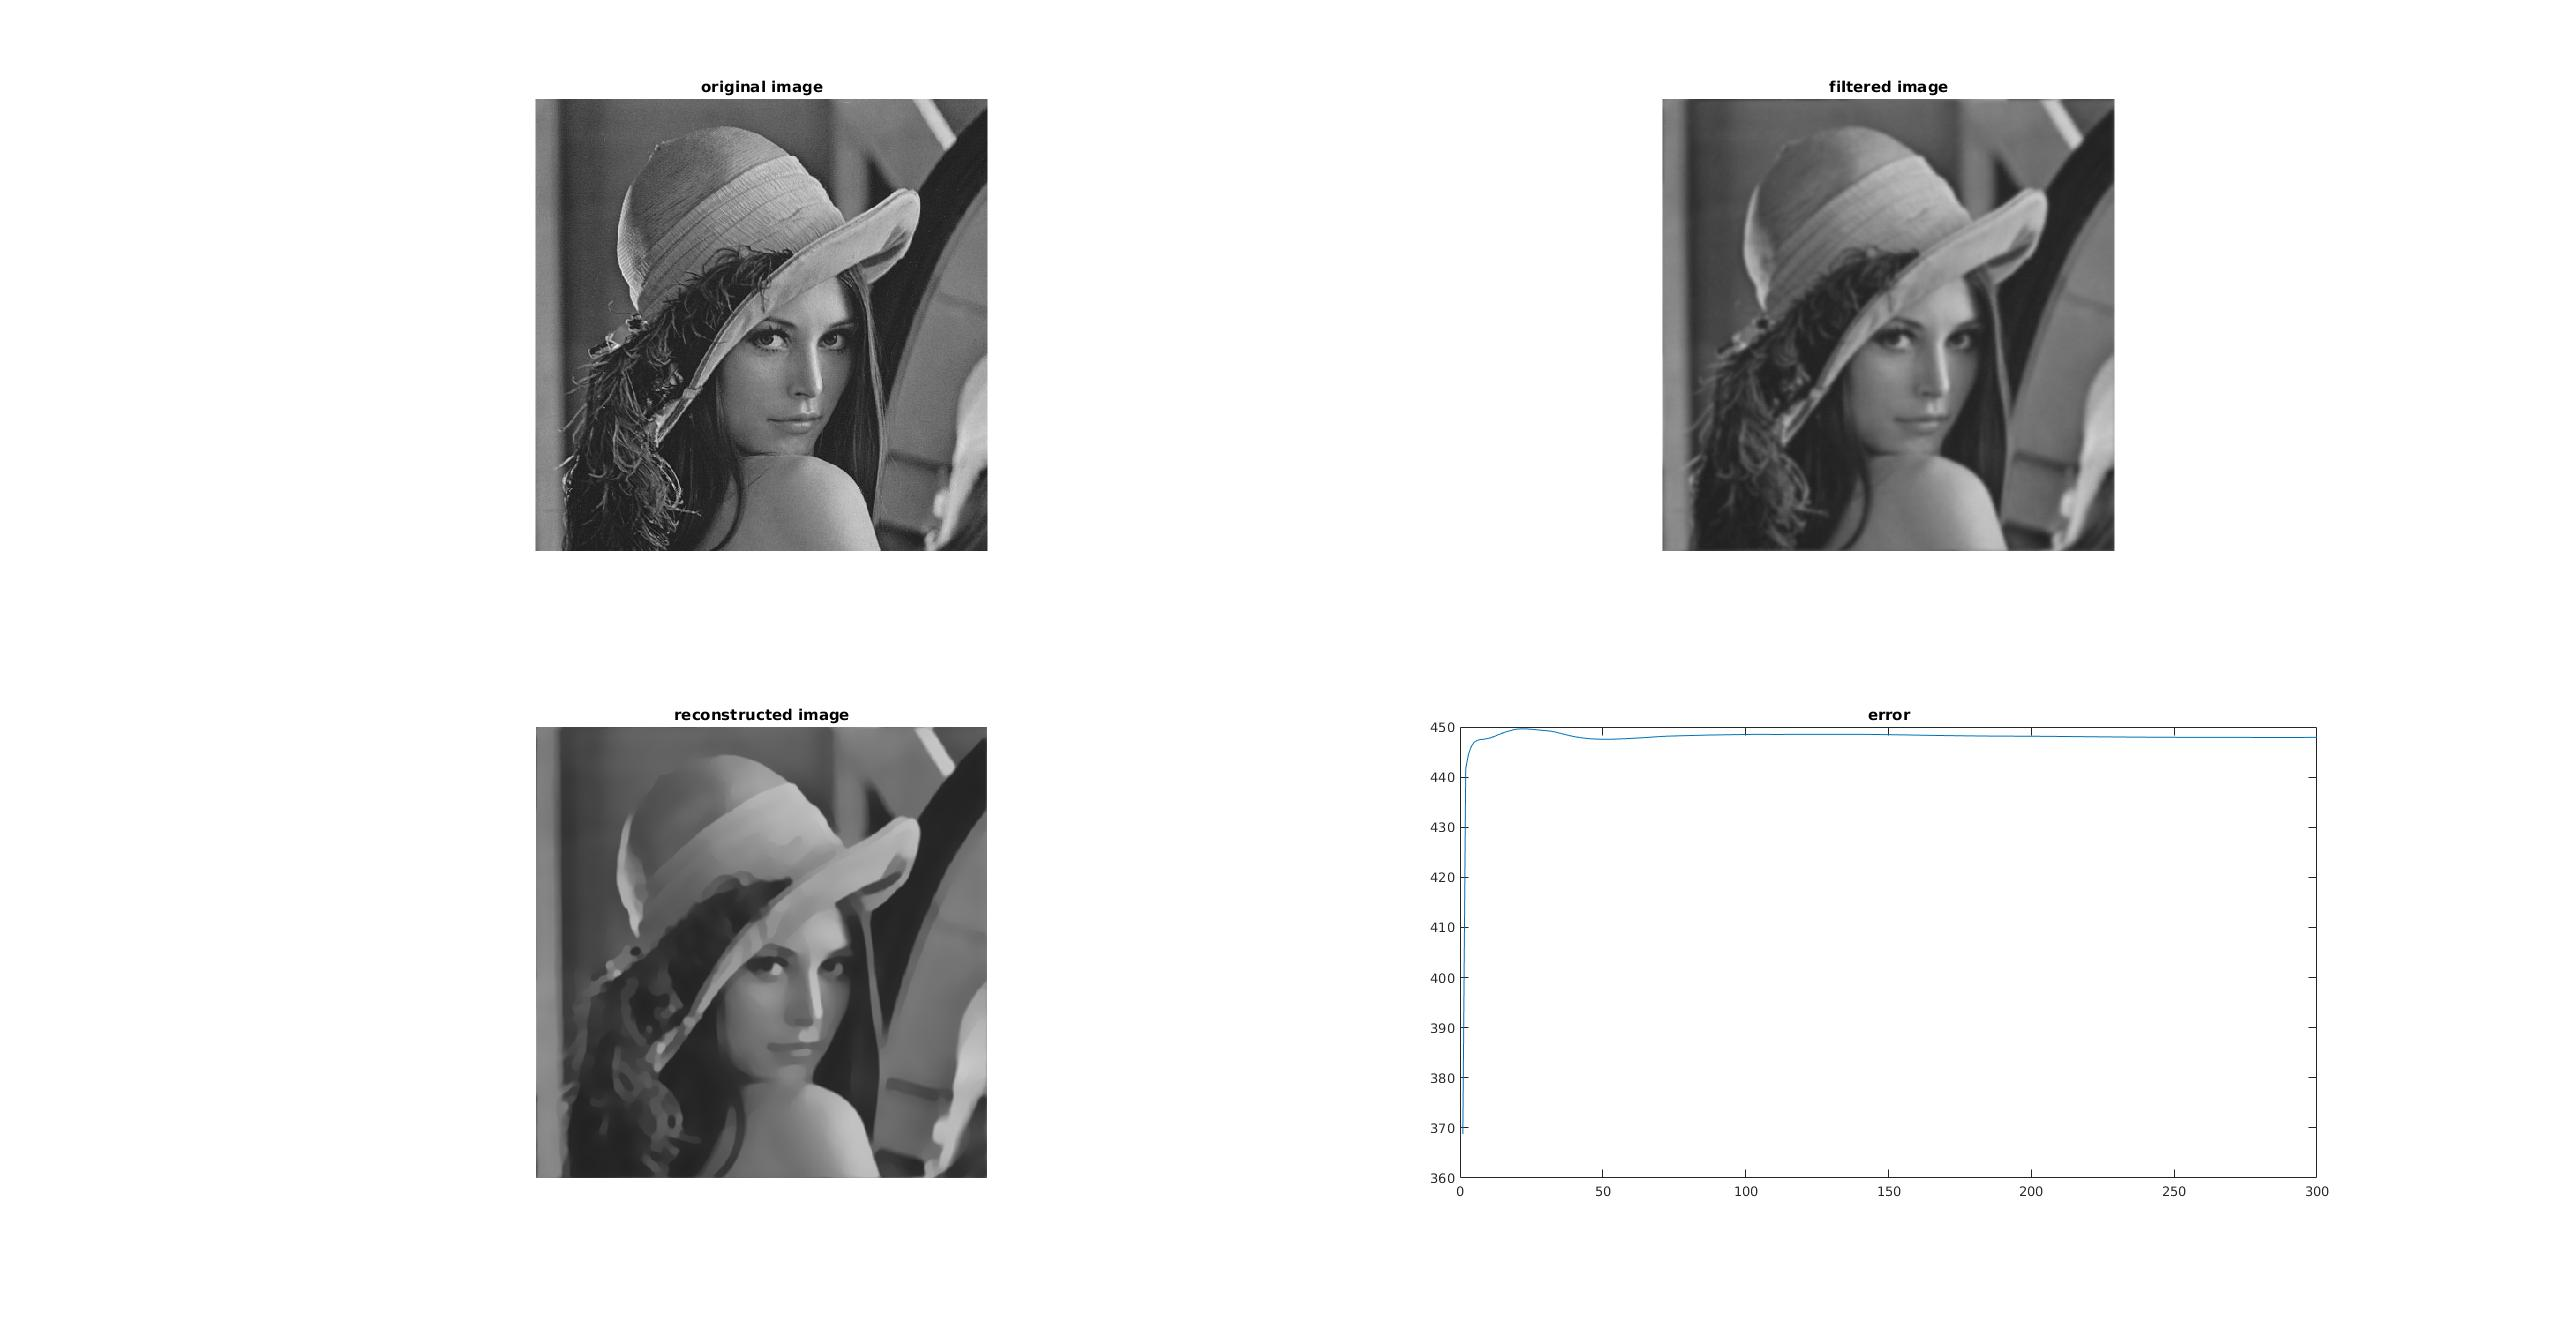
\includegraphics[width = 1 \textwidth]{fig8.jpg}
					\caption{SIGMA=2.0,SCALE=200 数值实验结果}
				\end{figure}
				\begin{figure}[htbp!]
					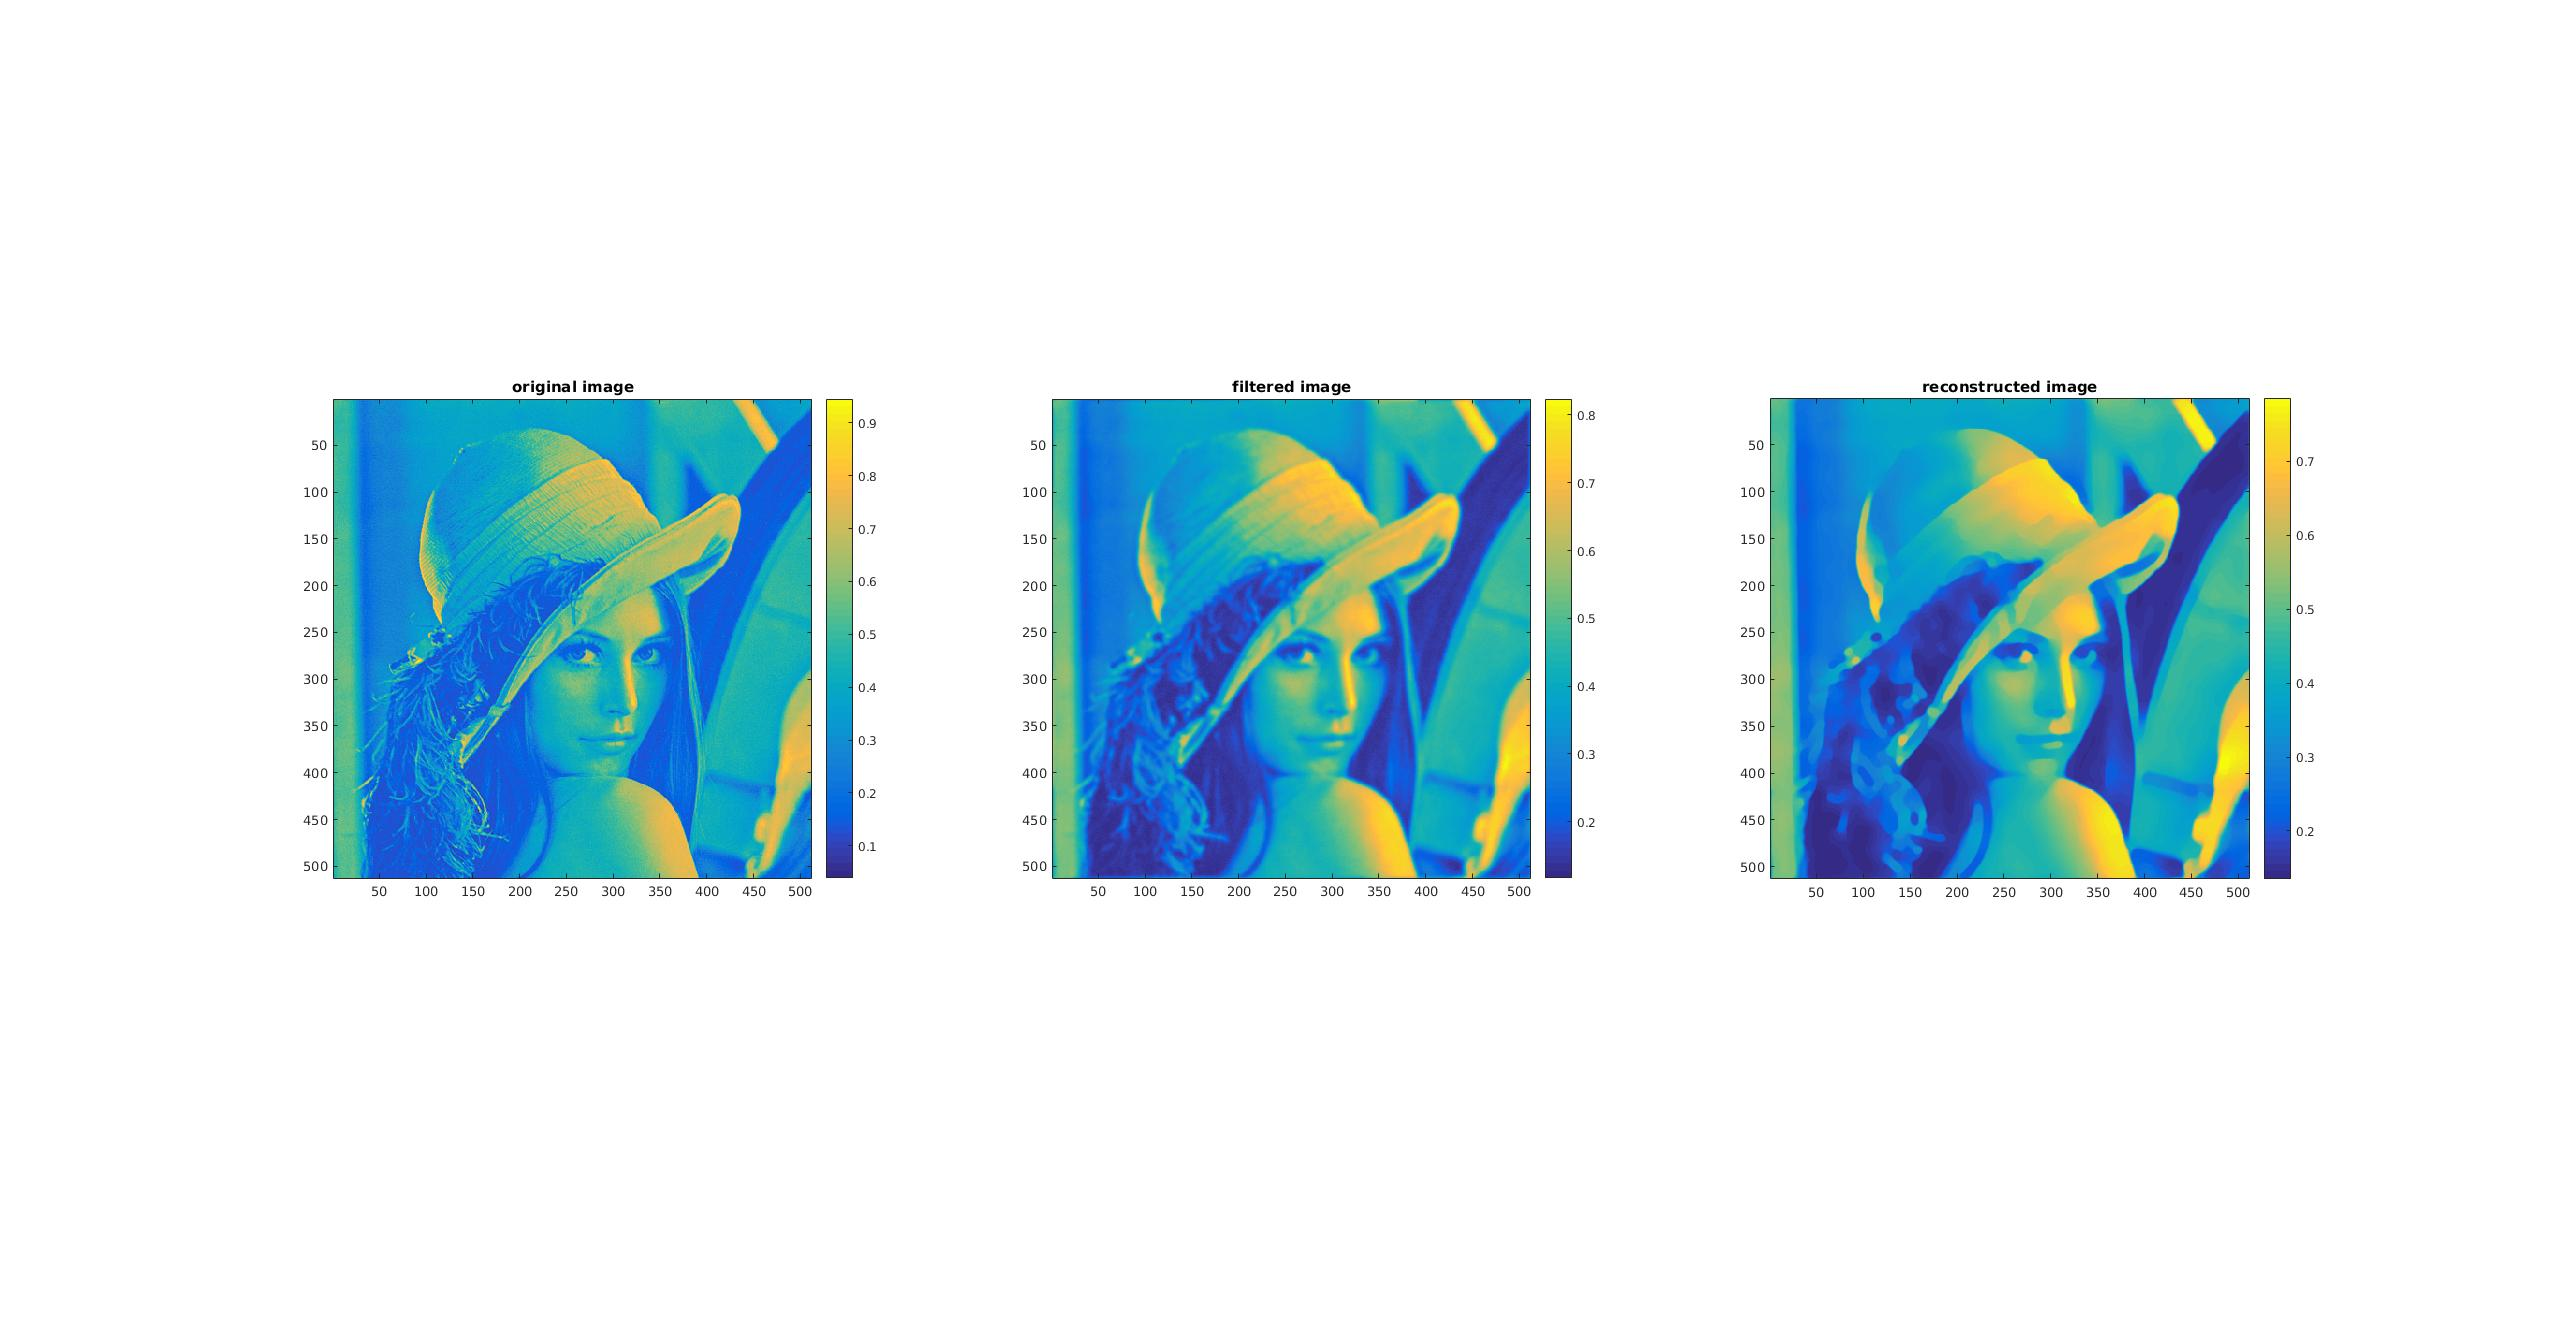
\includegraphics[width = 1 \textwidth]{fig9.jpg}
					\caption{SIGMA=2.0,SCALE=200 数值实验结果}
				\end{figure}
			\section{结论}
			\begin{enumerate}
				\item 从数值实验的结果来看,SIGMA的取值直接影响到了最终的误差结果,SIGMA=2.0时的误差显著大于SIGMA=1.5时的情形,与此同时,SCALE对最终误差的结果影响不大;
				\item 每一次数值实验的误差都经历了先增后降或先增后稳定的过程,这是由于我将filtered image设置为了迭代初始值,由此可以发现,从信息论的角度,ADMM算法的迭代过程并没有增加信息量,反而损失了图像的信息,这与图像处理的本质,即:“图像处理不会增加图像的信息量,只会使得图像中的一部分信息更为显著”相一致;
				\item 从恢复之后的图像可以看出,恢复之后的图像明显在皮肤、帽子、背景等平滑处均优于filtered image,在边缘处也起到了很好的保留边缘的作用,这与我们在算法中进行正则约束的目的是一致的,即算法实现达到了算法的设计目的;
				\item 算法的处理使得图像的信噪比提高,对比度显著增强,这是ADMM算法的优势;
				\item 从图像中头发区域的恢复情况可以看出,这一算法没有办法对原本已经丢失的细节进行恢复,这与我们的直观认识是一致的,即图像处理不会凭空产生细节,这是这一算法值得改进的地方;
			\end{enumerate}
\end{document}
